\subsection{Traffic Manager}

\includegraphics[width=0.9\linewidth]{../../img/frontend.pdf}

Sitting between the key-value store accelerator and the NIC is the traffic
manager, which routes network packets between the accelerator and the CPU.
Packets from the network card are first written into the main buffer.
At the same time, the controller inspects the packet header to determine if
the packet is a Memcached GET packet. If it is not a GET request, the packet
is sent on to the DMA engine. If it is, the key is sent to the accelerator and
the packet is moved from the main buffer to a defer buffer, allowing the
traffic manager to process subsequent packets without waiting for the result
to come back from the accelerator.

If a result does come back, the deferred packet is removed from the buffer and
the responder unit constructs a response by adding the necessary headers and
computing the IP and UDP checksums. The response is then sent back to the NIC.
If a zero-length result is returned, indicating that the key was not found in
the accelerator, the deferred is packet is sent on to the DMA engine.

The traffic manager also takes outbound packets from the DMA engine. An arbiter
is used to interleave transmission of these packets with transmission of
memcached response packets from the accelerator.
